% --------------------------------------------------------------- %
%             3. IOTA PANAUDOJAMUMAS TIEKIMO GRANDINĖSE 
% --------------------------------------------------------------- %

\section{IOTA panaudojamumas tiekimo grandinėse}

Prieš pradėdami modeliuoti IOTA taikymą, turime apsibrėžti sąlygas, kada tą apsimokėtų daryti. Technologiją galime taikyti bet kurioje tiekimo grandinėje, kuri tenkina bent vieną sąlygą:
\begin{itemize}
    \item Reikalingi jutikliais arba kitais prietaisais pamatuojami duomenys, pavyzdžiui RFID jutiklis, matuojantis temperatūrą konteineryje.
    \item Atliekamos finansinės arba informacinės transakcijos. Pavyzdžiui, atsiskaitoma už paslaugas ar prekes.
    \item Reikalingas automatizuotas M2M bendravimas. Pavyzdžiui, vieni elektroniniai prietaisai bendrauja ar perduoda informaciją kitiems prietaisams be papildomo žmogaus įsikišimo.
    \item Reikalingas absoliutus duomenų nekintamumas, t.y. kad duomenų negalėtų pakoreguoti ar ištrinti absoliučiai niekas ir jie būtų prieinami amžinai.
    \item Reikalingi atlikti skaičiavimai, pavyzdžiui matematinės ir statistinės formulės priklausomai nuo daviklių duomenų.
\end{itemize}

Tiekimo grandinės atvejis buvo kuriamas šio darbo autoriaus, remiantis kelių šaltinių pavyzdinėmis idėjomis \cite{christopher2016logistics} \cite{webber2009building} \cite{patrick2017continuous} \cite{justin2016customer} ir sujungus jas į vieną bendrą diagramą. Diagrama nebuvo siekiama pavaizduoti realaus pasaulio tiekimo grandinės pavyzdžio\footnote{Dėl konfidencialumo priežasčių įmonės nėra linkusios skelbti oficialių savo tiekimo grandinių modelių.}, o labiau siekta sukurti modelį, apimantį kuo daugiau skirtingų tiekimo grandinės fazių ir etapų, kad tai leistų geriau atskleisti IOTA technologijos panaudojamumą. Autoriaus nuomone modelis galėjo būti dar detalesnis, tačiau tai neatspindėtų norimos perteikti esmės.



% --------------------------------------------------------------- %
%                   3.1. TIEKIMO GRANDINĖS ATVEJIS
% --------------------------------------------------------------- %

\subsection{Tiekimo grandinės atvejis}

Pabandykime sumodeliuoti paprastą tiekimo grandinę, kuri galėtų savo skirtinguose grandies etapuose būti praplėsta pritaikant naujas technologijas. Tokia tiekimo grandinė pavaizduota priede nr. 1. Šis teikimo grandinės atvejis vaizduoja supaprastintą vaisių tiekimo grandinę nuo sėklų įsigijimo iki kliento vaisių įsigijimo prekybos centre. Tiekimo grandinė išskaidyta į 15 diskrečių etapų, kurių kiekvienas aprašytas toliau:
\begin{enumerate}
    \item Ūkininkas superka sėklas iš tiekėjo. Prieš tai yra sudaromas raštiškas kontraktas tarp sėklų tiekėjo ir ūkininko, kad už tam tikrą kainą ūkininkas gaus tam tikrą kiekį sėklų. Be to, sutartyje gali būti papildomų sąlygų, jei sėklų tiekėjas laiku neturės sėklų arba jų kokybė neatitiks keliamų standartų.
    \item Ūkininkas nurenka pasėtą derlių. Tačiau prieš tai ūkininkas pasėja vaisių sėklas, sudaro tinkamas sąlygas jų auginimui, naudoja specialias trąšas ir atėjus laikui vaisius nurenka ir sandėliuoja.
    \item Ūkininkas parduoda derlių supirkėjui. Pardavimas vyksta pagal iš anksto sudarytą kontraktą. Ūkininkas įsipareigoja atėjus konkrečiam terminui parduoti atitinkamą kiekį vaisių, atitinkančių nustatytą kokybės standartą už atitinkamą kainą tiekėjui.
    \item Kurjeris pakrauna vaisius į sunkvežimį. Supirkėjas gali samdyti kurjerį iš logistikos įmonės, teikiančios transportavimo paslaugas arba turėti savo darbuotojus, atsakingus už prekių transportavimą. Pirmuoju atveju būtų sudaromas kontraktas tarp supirkėjo ir logistikos įmonės, įsipareigojančios atgabenti nepažeistas prekes iki nustatyto termino.
    \item Vaisiai transportuojami iki fabriko.
    \item Vaisiai apdirbami (pagaminami jų sub-produktai) ir sandėliuojami. Priklausomai nuo vaisių supirkėjo veiklos srities, jis gali vaisius paruošti pardavimui, pvz. apipurkšti cheminiu produktu, suteikiantį blizgumą ar ilgalaikiškumą, taip pat apdirbti juos supjaustant, panaudojant kaip sudedamąją dalį kituose produktuose ir t.t. Šie produktai sandėliuojami fabriko patalpose, kol atvyks kurjeriai, atsakingi už prekių transportavimą į prekybos centrus. Su prekybos centrais yra pasirašomi kontraktai, nustatantys kokius produktus už kokią kainą vaisių supirkėjas parduos prekybos centrui.
    \item Apdirbti vaisiai pakraunami į sunkvežimį. Čia kurjeris gali būti samdomas tuo pačiu principu, kaip ir 4 etape.
    \item Vaisiai transportuojami į jūrų uostą. Jūrų uostas pagal vidines taisykles perima konteinerį ir paruošia jį pakrovimui į laivą.
    \item Vaisių konteineriai pakraunami į krovininį laivą.
    \item Krovininis laivas nuplaukia į kitą uostą.
    \item Vaisių konteineriai iškraunami į sunkvežimius. Tikėtina, kad kurjeris yra iš tos pačios logistikos kompanijos, kurios sunkvežimis nuvežė konteinerį į pirmąjį jūrų uostą.
    \item Sunkvežimiai išvežioja vaisius į skirtingas šalis. Iki pasiekiant kitos valstybės sieną, kur kurjeris susiduria su muitine.
    \item Muitinėse patikrinami kroviniai. Priklausomai nuo valstybės, už krovinio įvežimą į šalį, gali būti taikomi skirtingi mokesčiai. Už atsiskaitymą yra atsakingas prekybos centras, norintis įsivežti prekes. Susimokėjus muitinė išduoda specialų leidimą.
    \item Vaisiai išvežiojami į prekybos centrus.
    \item Vaisiai parduodami galutiniams pirkėjams.
\end{enumerate}



% --------------------------------------------------------------- %
%   3.2. TIEKIMO GRANDINĖS ATVEJIS PRITAIKIUS IOTA TECHNOLOGIJĄ
% --------------------------------------------------------------- %

\subsection{Tiekimo grandinės atvejis pritaikius IOTA technologiją}

Pasinaudodami 2.2.2. skyriaus ir jo poskyriuose nurodytomis IOTA savybėmis, galime apsibrėžti, kokius tiekimo grandinės procesus galima pagerinti ir kaip. Kiekvienas panaudojimo atvejo etapas arba etapai aprašyti atskirai, pateikiant diagramą su kiekvieno punkto detaliu aprašymu.



% --------------------------------------------------------------- %
%   3.2.1 PIRMAS ETAPAS
% --------------------------------------------------------------- %

\subsubsection{Pirmas etapas}

1 atvejis, „Ūkininkas superka sėklas iš tiekėjo“, pavaizduotas 12 pav.
\begin{enumerate}
    \item Tarp sėklų pardavėjo ir ūkininko yra sudaromas kontraktas, kad už tam tikrą sumą tam tikru metu ūkininkas galės įsigyti tam tikrą kiekį sėklų. Kontraktas pasirašomas ūkininko ir sėklų tiekėjo, o elektroninė sandorio versija užšifruojama raktu ir gautas šifras patalpinamas į IOTA raizginį. Abi šalys gauna dokumento kopiją ir šifro raktą. Niekas iš IOTA tinklo narių, išskyrus abi kontrakto šalis, negali peržiūrėti kontrakto turinio. Kontrakto šalys gali įrodyti turimos kontrakto kopijos autentiškumą užšifruodami šią kopiją ir patikrindami gauto šifro reikšmę su raizginyje esančiu šifru.
    \item Sėklų tiekėjas IOTA raizginyje sukuria MAM kanalą, kurį užsiprenumeruoja ūkininkas. Kanalu perduodami duomenys rašomi į raizginį, o ūkininkas gali stebėti sėklų būseną, pavyzdžiui lokaciją, sandėliavimo sąlygas ir pan.
    \item Sėklų tiekėjas pristato sėklas ūkininkui, o ūkininkas atlieką finansinį pavedimą tiekėjui.
\end{enumerate}

\begin{figure}[H]
    \centering
    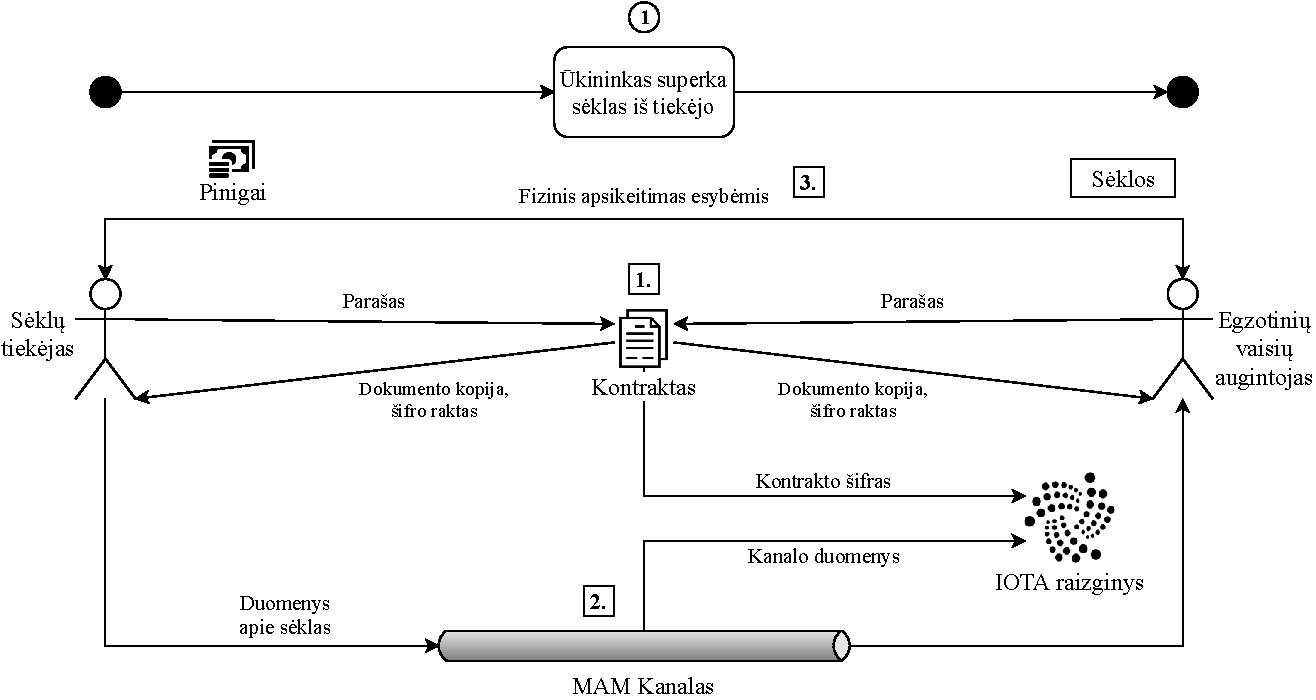
\includegraphics[scale=0.7]{images/iota-usecase-1}
    \caption{Panaudojimo atvejo 1 etapas}
\end{figure}



% --------------------------------------------------------------- %
%   3.2.2 ANTRAS ETAPAS
% --------------------------------------------------------------- %

\subsubsection{Antras etapas}

2 atvejis, „Ūkininkas nurenka pasėtą derlių“, pavaizduotas 13 pav.
\begin{enumerate}
    \item Iš pradžių ūkininkas inicijuoja MAM kanalą, kuriuo siųs duomenis potencialiems derliaus supirkėjams.
    \item Ten, kur yra pasodintos sėklos, pastatomi RFID jutikliai, siunčiantys kanalu duomenis apie auginimo sąlygas: drėgmę, temperatūrą ir kt.
    \item Esant poreikiui, specialūs IOTA orakulų rolę prisiėmę inspektoriai gali atlikti patikrą, ar RFID siunčiami duomenys nėra klastojami ir savo matavimus taip pat patalpinti IOTA raizginyje. Specialūs orakulai galėtų prisidėti ir prie kitų reikalavimų laikymosi patikros. Pavyzdžiui, ar ūkininkas auginimo metu neteršia aplinkos, nėra darbinami vaikai ir t.t. Orakulai gali prisidėti ir prie draudimo įmonių veiklos. Esant sausrai ir ūkininkui nepristačius pakankamai derliaus, draudimo kompanijos, gavusios patvirtinimą iš orakulų apie stichinę nelaimę, galėtų padengti ūkininkų nuostolius.
\end{enumerate}

\begin{figure}[H]
    \centering
    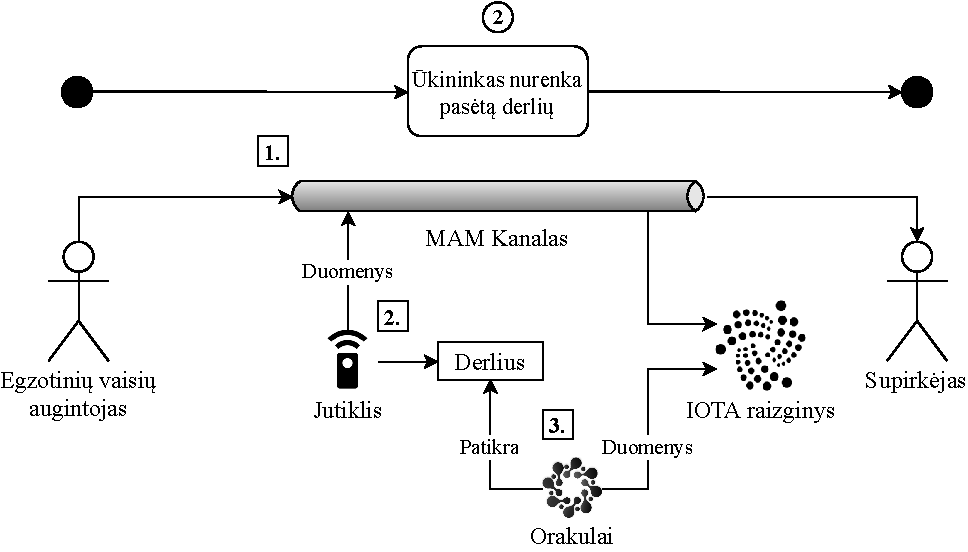
\includegraphics[scale=0.7]{images/iota-usecase-2}
    \caption{Panaudojimo atvejo 2 etapas}
\end{figure}



% --------------------------------------------------------------- %
%   3.2.3 TREČIAS ETAPAS
% --------------------------------------------------------------- %

\subsubsection{Trečias etapas}

3 atvejis, „Ūkininkas parduoda derlių supirkėjui“, yra beveik identiškas 1 atvejui. Šiuo atveju kontraktas tarp ūkininko ir supirkėjo gali būti sudaromas prieš 2, o esant poreikiui ir prieš 1 etapą tam, kad būtų galima sekti įsipareigojimų vykdymą.



% --------------------------------------------------------------- %
%   3.2.4 KETVIRTAS IR PENKTAS ETAPAI
% --------------------------------------------------------------- %

\subsubsection{Ketvirtas ir penktas etapai}

4 ir 5 atvejai, „Kurjeris pakrauna vaisius į sunkvežimį“ ir „Vaisiai transportuojami iki fabriko“, pavaizduoti 14 pav.
\begin{enumerate}
    \item Pakrovęs vaisius į sunkvežimį kurjeris sukuria MAM kanalą šitaip patvirtinantis perėmęs krovinį. MAM kanalą prenumeruoja fabrikas (supirkėjas).
    \item Į MAM kanalą yra perduodami duomenys iš RFID įrenginio apie sunkvežimyje esančio krovinio sąlygas ir sunkvežimio lokaciją. Fabrikui\footnote{Šiame panaudojimo atvejo pavyzdyje fabrikas priklauso supirkėjui.} tai yra naudinga, nes fabrikas gali reaguoti į vaisių atvežimą, pasiruošti jam. Be to, jei vaisiai vėluotų, dingtų bei būtų pristatyti pažeisti arba neatitinkantys kokybės, būtų aišku kur tai įvyko ir kas yra kaltininkas.
    \item Vaisiai pristatomi į fabriką, kur yra perduodama atsakomybė už juos\footnote{Paprastai kaskart atlikus transakciją perduodant krovinį, kartu perduodama ir atsakomybė už jį. Tai reiškia, kad krovinį perimanti šalis turi patikrinti krovinio būklę, kad galėtų atrasti pažeidimo priežastį ir kaltininką.}.
\end{enumerate}

\begin{figure}[H]
    \centering
    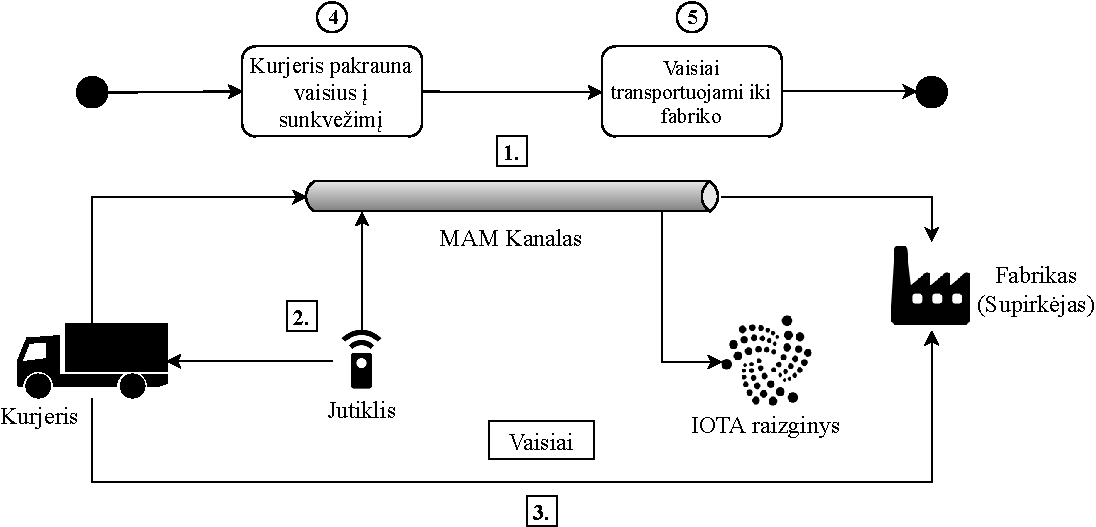
\includegraphics[scale=0.7]{images/iota-usecase-4-5}
    \caption{Panaudojimo atvejo 4 ir 5 etapai}
\end{figure}



% --------------------------------------------------------------- %
%   3.2.5 ŠEŠTAS ETAPAS
% --------------------------------------------------------------- %

\subsubsection{Šeštas etapas}

6 atvejis, „Vaisiai apdirbami (pagaminami jų sub-produktai) ir sandėliuojami“, pavaizduoti 15 pav.
\begin{enumerate}
    \item Kaip ir pirmame panaudojimo atvejo etape, yra sudaromas kontraktas. Fabrikas (supirkėjas) susitaria su prekybos centru, kad už tam tikrą sumą tam tikru metu bus parduotas tam tikras kiekis perdirbtų arba paruoštų vaisių. Kontraktas pasirašomas abiejų šalių, o elektroninė versija užšifruojama raktu ir gautas šifras patalpinamas į IOTA tinklą \footnote{Kontraktas gali būti sudarytas gerokai anksčiau, pavyzdžiui prieš 1 arba 2 etapą}. Niekas iš IOTA tinklo narių, išskyrus abi kontrakto šalis, negali peržiūrėti kontrakto turinio. Kontrakto šalys gali įrodyti turimo kontrakto teisiškumą užšifruodami šią kopiją ir patikrindami gauto šifro reikšmę su raizginyje esančiu šifru.
    \item Fabrikas sukuria kanalą, kurį prenumeruoja prekybos centrai\footnote{Jeigu krovinius transportuoja samdomi kurjeriai iš logistikos įmonių, kanalu duomenys gali būti siunčiami ir šiems atstovams, t.y. koks krovinių tipas, kada krovinys paruoštas transportavimui ir t.t.}. Kanalu fabrikas perduoda informaciją apie tai, kokie produktai kuriami, kurioje gamybos stadijoje, kokiais standartais apdirbami ir t.t.
    \item Fabrike įtaisyti RFID jutikliai kanalu taip pat perduoda informaciją: gamybos sąlygas skirtinguose etapuose.
    \item Esant poreikiui inspektoriai, kitaip orakulai, gali patikrinti tiek 2, tiek 3 žingsnyje fabriko teikiamą informaciją ir patalpinti į IOTA raizginį prekybos centrams patikrinti.
\end{enumerate}

\begin{figure}[H]
    \centering
    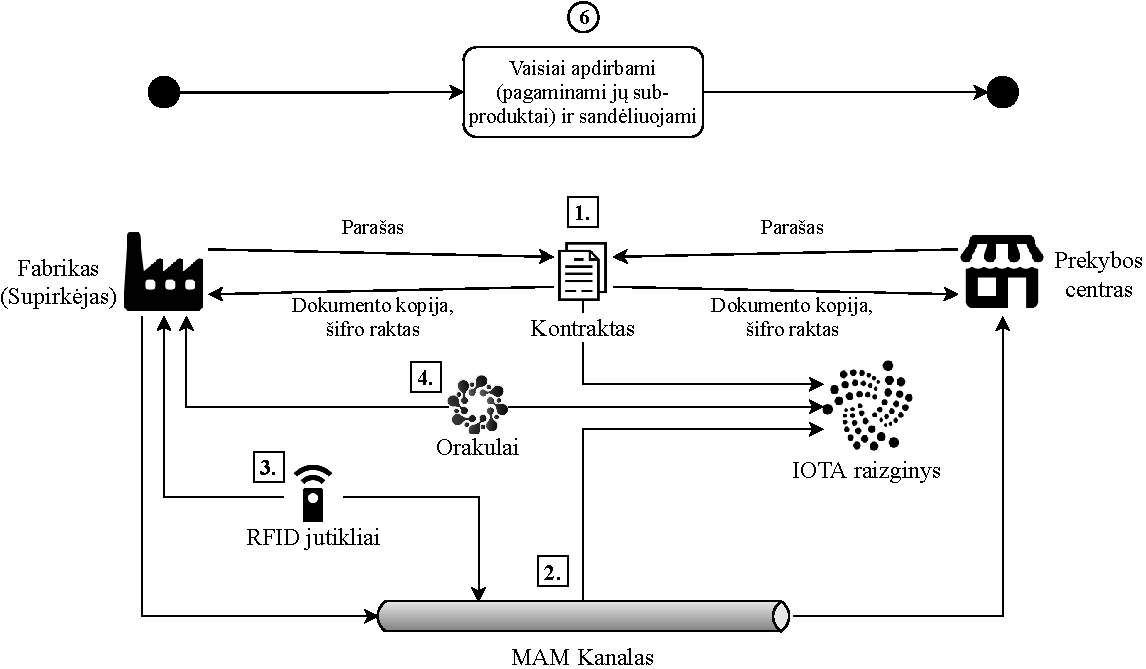
\includegraphics[scale=0.7]{images/iota-usecase-6}
    \caption{Panaudojimo atvejo 6 etapas}
\end{figure}



% --------------------------------------------------------------- %
%   3.2.6 SEPTINTAS IR AŠTUNTAS ETAPAI
% --------------------------------------------------------------- %

\subsubsection{Septintas ir aštuntas etapai}

7 ir 8 atvejai, „Apdirbti vaisiai pakraunami į sunkvežimį“ ir „Vaisiai transportuojami į jūrų uostą“, yra beveik identiški atitinkamai 4 ir 5 atvejui. Kurjeriui atidarius kanalą, jį prenumeruoja ne tik prekybos centras, bet ir jūrų uostas, kad būtų pasiruošta sunkvežimio atvykimui.



% --------------------------------------------------------------- %
%   3.2.7 DEVINTAS IR DEŠIMTAS ETAPAI
% --------------------------------------------------------------- %

\subsubsection{Devintas ir dešimtas etapai}

9 ir 10 atvejai, „Vaisių konteineriai pakraunami į krovininį laivą“ ir „Krovininis laivas nuplaukia į kitą uostą“, pavaizduoti 16 pav.
\begin{enumerate}
    \item Vaisiai pakraunami į krovininį laivą.
    \item Laivas sukuria MAM kanalą, kurį užprenumeruoja kurjeris, laukiantis krovinio jūrų uoste nr. 2. Kanalu perduodama konteinerio su vaisiais laikymo sąlygos, gaunamos iš RFID jutiklių. Laivas išplaukia iš jūrų uosto nr. 1
    \item Laivui plaukiant jūra, dingsta interneto ryšys, tačiau informacijos tiekimas nenutraukiamas ir daromos informacijos transakcijos neprisijungus. 
    \item Po kiek laiko interneto ryšys grįžta ir visas iki tol siųstas žinutes prenumeruotojas gali gauti ir matyti iškart.
    \item Vaisiai transportuojami į jūrų uostą nr. 2.
\end{enumerate}

\begin{figure}[H]
    \centering
    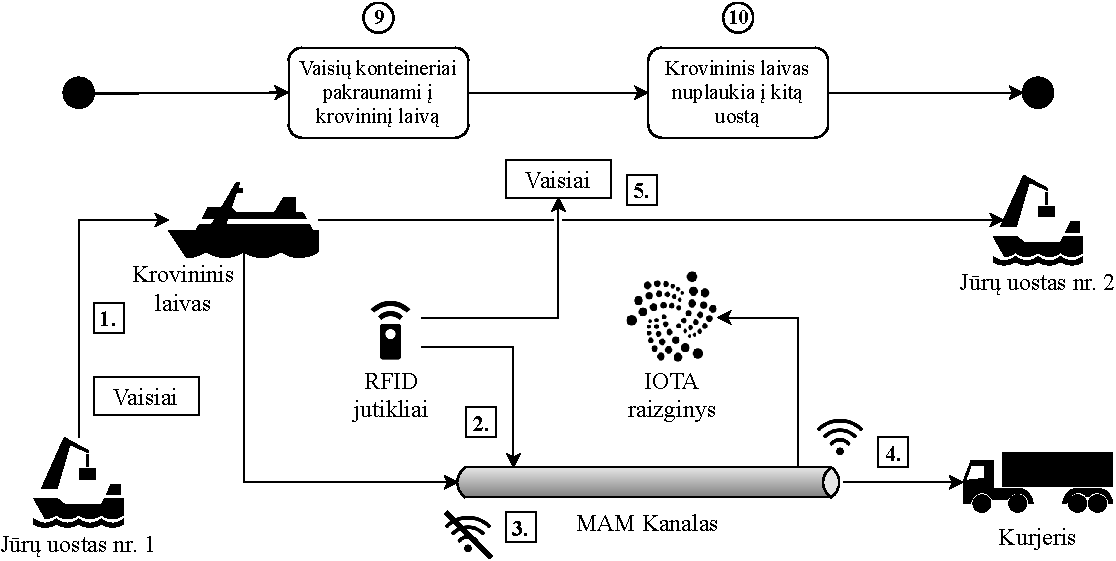
\includegraphics[scale=0.7]{images/iota-usecase-9-10}
    \caption{Panaudojimo atvejo 9 ir 10 etapai}
\end{figure}



% --------------------------------------------------------------- %
%   3.2.8 VIENUOLIKTAS IR DVYLIKTAS ETAPAI
% --------------------------------------------------------------- %

\subsubsection{Vienuoliktas ir dvyliktas etapai}

11 ir 12 atvejai, „Vaisių konteineriai iškraunami į sunkvežimius“ ir „Sunkvežimiai išvežioja vaisius į skirtingas šalis“, pavaizduoti 17 pav.
\begin{enumerate}
    \item Jūrų uoste nr. 2 iškraunamas konteineris su vaisiais, kurį perima kurjeris.
    \item Kurjeris sukuria MAM kanalą, kurį užprenumeruoja Prekybos centras.
    \item Kurjeris galiausiai pasiekia kitos valstybės muitinę.
\end{enumerate}

\begin{figure}[H]
    \centering
    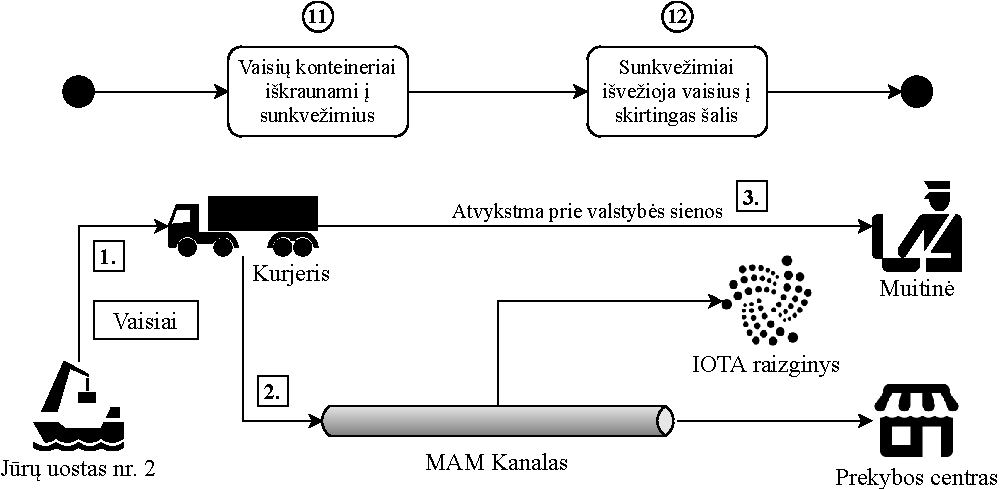
\includegraphics[scale=0.7]{images/iota-usecase-11-12}
    \caption{Panaudojimo atvejo 11 ir 12 etapai}
\end{figure}



% --------------------------------------------------------------- %
%   3.2.9 TRYLIKTAS ETAPAS
% --------------------------------------------------------------- %

\subsubsection{Tryliktas etapas}

13 atvejis, „Muitinėse patikrinami kroviniai“, pavaizduotas 18 pav.
\begin{enumerate}
    \item Kurjeris perduoda vaisių konteinerį muitinės darbuotojų patikrai.
    \item Muitinės darbuotojai patikrina vaisių kelionės gyvavimo ciklo informaciją IOTA raizginyje. Ši informacija leidžia muitinės darbuotojams lengvai patikrinti svarbią informaciją. Pavyzdžiui, JAV pasienio muitų įstatymas įpareigoja pateikti krovinio pirkėją, pardavėją, gamintoją, kilmės šalį ir kitus duomenis \cite{customs2018importer}, kuriuos galima atsekti IOTA raizginyje. 
    \item Muitinės darbuotojams neradus nieko įtartino, suteikiamas leidimas krovinį įvežti į valstybę. Vaisius transportuojanti valstybė susimoka muito mokestį (jeigu toks yra taikomas).
\end{enumerate}

\begin{figure}[H]
    \centering
    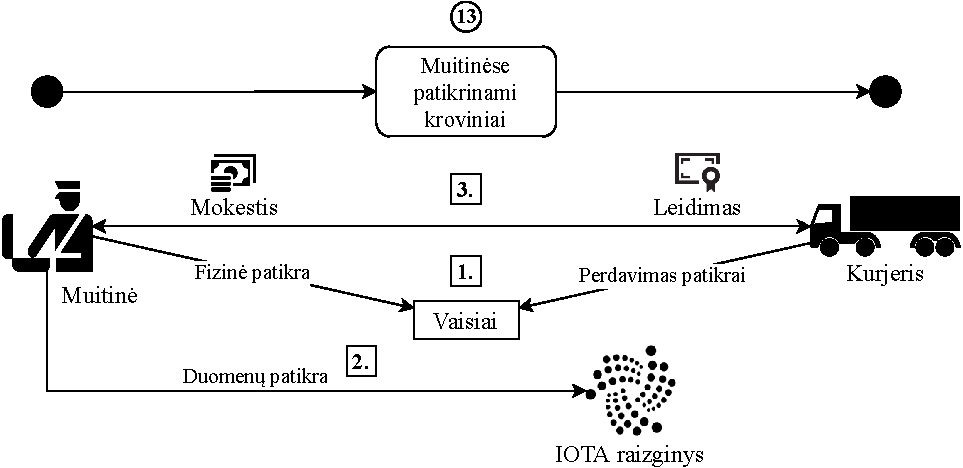
\includegraphics[scale=0.7]{images/iota-usecase-13}
    \caption{Panaudojimo atvejo 13 etapas}
\end{figure}



% --------------------------------------------------------------- %
%   3.2.10 KETURIOLIKTAS IR PENKIOLIKTAS ETAPAI
% --------------------------------------------------------------- %

\subsubsection{Keturioliktas ir penkioliktas etapai}

14 ir 15 atvejai, „Vaisiai išvežiojami į prekybos centrus“ ir „Vaisiai parduodami galutiniams pirkėjams“, pavaizduoti 18 pav.
\begin{enumerate}
    \item Vaisiai transportuojami į prekybos centrą, kuriame šie yra paruošiami pardavimui klientams.
    \item Prekybos centrų klientai nusiperka vaisių pakuotes už tam tikrą kainą.
    \item Pirkėjas gali įsitikinti prekybos centro pateikiama informacija, nuskenavęs ant pakuotės esantį QR kodą. Speciali programėlė galėtų leisti peržiūrėti kilmės šalį, vaisių kelionės maršrutą, vaisių auginimo, sandėliavimo ir transportavimo sąlygas, taip pat bet kokią papildomą informaciją, kurią tiekėjai gali atskleisti pirkėjui. Visa ši informacija gaunama iš IOTA raizginyje MAM kanalais bei kitais būdais patalpintos informacijos.
\end{enumerate}

\begin{figure}[H]
    \centering
    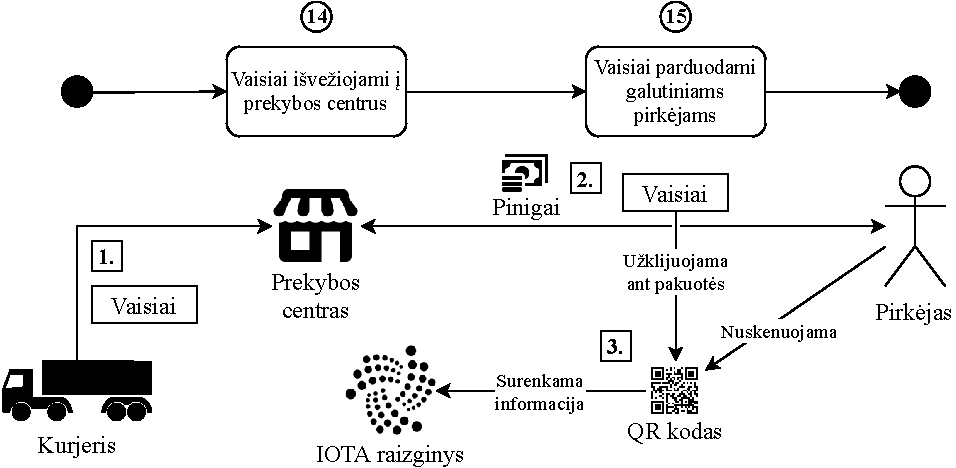
\includegraphics[scale=0.7]{images/iota-usecase-14-15}
    \caption{Panaudojimo atvejo 14 ir 15 etapai}
\end{figure}